
%(BEGIN_QUESTION)
% Copyright 2005, Tony R. Kuphaldt, released under the Creative Commons Attribution License (v 1.0)
% This means you may do almost anything with this work of mine, so long as you give me proper credit

Linemen working on high-voltage conductors do not simply rely on open disconnect switches to isolate sections of power lines from sources of electricity during maintenance.  They also attach ``grounding'' cables from line to line, and then to earth ground like this:

$$\includegraphics[width=15.5cm]{i01860x01.eps}$$

Explain why this decreases the risk of electric shock for the linemen, based on what you know about {\it electrically common points} in a circuit.

\underbar{file i01860}
%(END_QUESTION)





%(BEGIN_ANSWER)

By connecting the three wires together, you make them electrically common to each other.  This prevents any substantial voltage (potential difference) developing between them.  Likewise, connecting the three wires to the earth makes them electrically common to the earth, preventing any substantial voltage from developing between any of the wires and ground.

\vskip 10pt

Follow-up question: after the linemen are done with their work, they remove the grounding wires from the power lines before they close the disconnect switches.  Explain why this is done, by describing the catastrophic consequences of closing the disconnect switches with the grounding wires still in place.

%(END_ANSWER)





%(BEGIN_NOTES)

A physicist would describe such a ``grounded'' system as being one large {\it equipotential surface}.  This is an important concept for students to grasp, not only for safety but also for the purpose of better understanding where voltage drops should and {\it should not} be in working circuits.

Some students may (wisely) ask how any voltage at all could be developed between the isolated conductors in the absence of grounding wires, since the disconnect switches are open at all points.  Although it may be premature to discuss with your students how capacitive coupling with nearby (energized) conductors could cause voltages to appear between non-grounded conductors and ground (depending on their level of electrical understanding), you can still answer the question by appealing to a general sense of safety conservatism.  With the wires all made electrically common to each other and to earth ground, there is still some measure of protection even in the event of one or more of the disconnect switches accidently closing, a lightning strike, or a bird landing between the open poles of a disconnect switch.

If your students have not yet studied three-phase AC systems, they may (wisely) ask why three power line conductors are necessary instead of two.  You may tell them that this is irrelevant to the safety question: that all they need to know is that there will be high voltage present between each wire pair (A and B, B and C, A and C) and between each wire and ground, when the power lines are in operation.

%INDEX% Safety, electrical: lock-out / tag-out and power line grounding

%(END_NOTES)


